\chapter{Properties}
\label{properties:sec}

The maspack property package ({\tt maspack.properties}) provides a
uniform means by which classes can export specific attributes and
information about them to application software.  The main purpose of
properties is to

\begin{enumerate}

\item Provide generic code for accessing and modifying attributes. 

\item Remove the need for "boiler-plate" code to read or write attributes
from persistent storage, or modify them by other means such as a GUI
panel.

\end{enumerate}

The property software uses Java reflection to obtain information about
a property's value and its associated class, in a manner similar to
that used by the properties of Java Beans.

\section{Accessing Properties}

Any class can export properties by implementing the
interface \javaclass[maspack.properties]{HasProperties}:

\begin{lstlisting}[]
interface HasProperties
{
   // get a handle for a specific named property
   Property getProperty (String name);

   // get a list of all properties associated with this class
   PropertyInfoList getAllPropertyInfo ();
}
\end{lstlisting}

Each property is associated with a name, which must be a valid Java
identifier. The
\javamethod[maspack.properties.HasProperties]{getProperty()} method returns
a \javaclass[maspack.properties]{Property} handle to the named property, 
which can in turn be
used to access that property's values or obtain other information
about it. \javamethod[maspack.properties.HasProperties]{getAllPropertyInfo()}
returns a \javaclass[maspack.properties]{PropertyInfoList}
providing information about all the properties associated with the
class.

A \javaclass[maspack.properties]{Property} handle supplies the following methods:
\begin{lstlisting}[]
interface Property
{
   Object get(); 
   void set (Object value); 
   Range getRange ();
   HasProperties getHost();
   PropertyInfo getInfo();
}
\end{lstlisting}

\begin{description}

\item[{\tt get()} ] \mbox{}

Returns the property's value. As a rule, returned 
returned values should be treated as read-only.

\item[{\tt set()} ] \mbox{}

Sets the property's value (unless it is read-only, see Section
\ref{propertyInfoSec}).

\item[{\tt getRange()} ] \mbox{}

Returns a {\tt Range} object for a property
(see Section \ref{rangesSec}), which is used to determine which values
are admissible to {\tt set}.  If all values are admissible, {\tt
getRange()} can return {\tt null}.

\item[{\tt getHost()} ] \mbox{}

Returns the object to which this property handle belongs.

\item[{\tt getInfo()} ] \mbox{}

Returns static information about this property (see Section
\ref{propertyInfoSec}).

\end{description}

A simple example of property usage is given below. Assume that we have
a class called {\tt DeformableModel} which contains a property called
{\tt stiffness}, and we want to set the stiffness to 1000. This
could be done as follows:
\begin{lstlisting}[]
   DeformableModel defo = new DeformableModel();    
   Property stiff = defo.getProperty("stiffness");

   stiff.set (1000.0); // (uses Java 1.5 autoboxing to turn
                       // 1000.0 into Double(1000.0)
\end{lstlisting}
Of course, {\tt DeformableModel} will likely have a method called
{\tt setStiffness} that can be used to set the stiffness directly, without
having to got through the {\tt Property} interface.  However, the
purpose of properties is not to facilitate attribute access within
specially constructed code; it is to facilitate attribute access
within {\it generic} code that is hidden from the user. For instance,
suppose I want to query a property value from a GUI. The GUI must
obtain the name of the desired property from the user (e.g., through a
menu or a text box), and then given only that name, it must go and
obtain the necessary information from the object exporting that
property.  A {\tt Property} allows this to be done in a manner
independent of the nature of the property itself.

\subsection{Why Property Handles?}

In theory, one could embed the methods of {\tt Property}
directly within the {\tt HasProperties} interface, using
methods with signatures like 
\begin{lstlisting}[]
   Object getPropertyValue (String name);

   void setPropertyValue (String name, Object value);
\end{lstlisting}
The main reason for not doing this is performance: a property handle
can access the attribute quickly, without having to resolve the
property's name each time. 

Each property handle contains a back-pointer to the object containing,
or {\it hosting}, the property, which can be obtained with the 
{\tt getHost()} method.

\label{rangesSec}
\section{Property Ranges}

A \javaclass[maspack.util]{Range} object supplies information about what values a
particular {\tt Property} can be set to. It contains the following
methods:

\begin{lstlisting}[]
interface Range
{
   boolean isValid (Object obj, StringHolder errMsg);
   Object projectToRange (Object obj);
   void intersect (Range range);
   boolean isEmpty();
}
\end{lstlisting}

\begin{description}

\item[{\tt isValid()} ] \mbox{}

Returns {\tt true} if {\tt obj} is a valid
argument to the property's {\tt set} method. The optional
argument {\tt errMsg}, if not {\tt null}, is used to return
an error message in case the object is not valid.

\item[{\tt makeValid()} ] \mbox{}

Trys to turn {\tt obj} into a valid argument for {\tt set()}. If
{\tt obj} is a valid argument, then it is returned directly. Otherwise,
the method tries to return an object close to {\tt obj} that is in the
valid range. If this is not possible, the method returns
{\tt Range.IllegalValue}.

\item[{\tt intersect()} ] \mbox{}

Intersects the current range with another range and
placed the result in this range. The resulting range should admit values
that were admissible by both previous ranges.

\item[{\tt isEmpty()} ] \mbox{}

Returns {\tt true} if this range has no admissible values.
This is most likely to occur as the result of an intersection
operation.

\end{description}

Possible usage of a range object is shown below:

\begin{lstlisting}[]
   Property prop = hostHost.get ("radius");
   Range range = prop.getRange();
   StringHolder errMsg = new StringHolder();
   double r;

   ...

   if (!range.isValid (r, errMsg)) {
      System.err.println ("Radius r invalid, reason: " {\tt  errMsg.value);
   }
   else {
      prop.set (r);
   }
\end{lstlisting}

Two common examples of {\tt Range} objects are 
\javaclass[maspack.util]{DoubleInterval} and
\javaclass[maspack.util]{IntegerInterval}, 
which implement intervals of double and integer
values, respectively.  Ranges are also {\tt Clonable}, which means that
they can be duplicated by calling {\tt range.clone()}.

\label{propertyInfoSec}
\section{Obtaining Property Information}

Additional information about a property is available through the
\javaclass[maspack.properties]{PropertyInfo} 
interface, which can be obtained using the
{\tt getInfo()} method of the property handle.  Information supplied by
{\tt PropertyInfo} is static with respect to the exporting class and
does not change (unlike the property values themselves, which do
change). Such information includes the property's name, whether or not
it is read-only, and a comment describing what the property does.

Some of the {\tt PropertyInfo} methods include:
\begin{lstlisting}[]
interface PropertyInfo
{
   // gets the name of this property
   String getName(); 

   // returns true if this property cannot be set
   boolean isReadonly();

   // returns a string description of the property
   String getDescription();

   // returns an optional format string describing how the 
   // property's values should be formatted when printed.
   String getPrintFormat();
 
   // returns the class associated with this property's value.
   Class getValueClass();

   // returns the class associated with this property's host
   Class getHostClass();

   // returns true if the properties value should be written
   // by the PropertyList write method.
   boolean getAutoWrite();

   // returns the conditions under which this property 
   // should be interactively edited.
   Edit getEditing();

   // Returns information about whether the property's editing widget
   // should be able to expand or contract in order to save GUI space. 
   ExpandState getWidgetExpandState();

   // Indicates if a slider is allowed in this property's editing
   // widget
   boolean isSliderAllowed();

   // returns the default value for this property
   Object getDefaultValue();

   // returns a default numeric range for this property, if any
   public NumericInterval getDefaultNumericRange();

   // writes a value of this object out to a PrintStream
   void writeValue (
       Object value, PrintWriter pw, NumberFormat fmt);

   // scans a value of this object from a ReaderTokenizer
   Object scanValue (ReaderTokenizer rtok);

   // creates a Property for this property, attached
   // to the specified host object
   Property createHandle (HasProperties host);

   // returns true if a specified value equals this
   // property's default value
   boolean valueEqualsDefault();

   // returns true if the property is inheritable
   boolean isInheritable();

   // returns the property's numeric dimension, or -1 if it
   // is not numeric or does not have a fixed dimension
   int getDimension();

   // indicates that the property value can be shared among
   // several hosts.
   boolean isSharable();
}
\end{lstlisting}

Property information can also be obtained directly from the exporting
class, using {\tt getAllPropertyInfo()}, which returns
information for all the properties exported by that class. This
information is contained within a 
\javaclass[maspack.properties]{PropertyInfoList}:
\begin{lstlisting}[]
interface PropertyInfoList
{
   // number of properties in this list
   int size(); 

   // returns an iterator over all the property infos
   Iterator<PropertyInfo> iterator();

   // returns info for a specific named property
   PropertyInfo get (String name);

   // returns true if this list has no inheritable properties
   boolean hasNoInheritableProperties();
}
\end{lstlisting}
For example, suppose we want to print the names of all the
properties associated with a given class. This could
be done as follows:
\begin{lstlisting}[]
   HasProperties exportingObject;
   ...
   PropertyInfoList infoList = 
       exportingObject.getAllPropertyInfo();
   for (PropertyInfo info : infoList) {
      System.out.println (info.getName());
   }
\end{lstlisting}

\label{exportingSec}
\section{Exporting Properties from a Class }

As indicated above, a class can export properties by implementing the
interface {\tt HasProperties}, along with the supporting interfaces
{\tt Property}, {\tt PropertyInfo}, and {\tt PropertyInfoList}.  The
class developer can do this in any way desired, but support is
provided to make this fairly easy.

The standard approach is to create a static instance of 
{\tt PropertyList} for the exporting class, and then populate it with
{\tt PropertyInfo} structures for the various exported properties. This
{\tt PropertyList} (which implements {\tt PropertyInfoList}) can then
be used to implement the {\tt getProperty()} and {\tt getAllPropertyInfo()} 
methods required by {\tt HasProperties}:
\begin{lstlisting}[]
   protected static PropertyList myProps;
 
   ... initialize myProps in a static code block ...

   // returns an information list for all properties
   public PropertyInfoList getAllPropertyInfo () {
      return myProps;
   }

   // returns a handle for a specific property
   public Property getProperty (String name) {
      getAllPropertyInfo().getProperty (name, this);
   }
\end{lstlisting}

Information about specific properties should be added to {\tt PropertyList} 
within a static code block (second line in the above
fragment). This can be done directly using the method
\begin{lstlisting}[]
   void add (PropertyInfo info)
\end{lstlisting}
but this requires creating and initializing a {\tt PropertyInfo}
object. An easier way is to use a different version of the {\tt add}
method, which creates the required {\tt PropertyInfo} 
structure based on information supplied through its
arguments.  In the example below, we have a class
called {\tt ThisHost} which exports three properties called {\tt visible}, 
{\tt lineWidth}, and {\tt color}:

\begin{lstlisting}[]
   // default values for the properties
   protected static int defaultLineWidth = 1;
   protected static boolean defaultVisibleP = true;
   protected static Color defaultColor = 
      new Color (0.5f, 0.5f, 0.5f);

   // fields containing the property values
   protected int myLineWidth = defaultLineWidth;
   protected boolean myVisibleP = defaultVisibleP;
   protected Color myColor = defaultColor;

   // create a PropertyList ...
   protected static PropertyList myProps = 
      new PropertyList(ThisHost.class);

   // ... and add information for each property:
   static {
      myProps.add (
         "visible isVisible *", "object is visible", 
          defaultVisibleP);
      myProps.add (
         "lineWidth", "line width (pixels)", 
         defaultLineWidth);
      myProps.add (
         "color", "color ", defaultColor);
   }

   public PropertyInfoList getAllPropertyInfo () {
      return myProps;
   }

   public Property getProperty (String name) {
      getAllPropertyInfo().get (name, this);
   }
\end{lstlisting}
The values for the three properties are stored in the fields {\tt myLineWidth}, 
{\tt myVisibleP}, and {\tt myColor}. Default values for
these are defined by static fields.

A static instance of a {\tt PropertyList} is created, using a
constructor which takes the exporting class as an argument (in Java
1.5, the class object for a class can be referenced as 
{\it ClassName}{\tt .class}). Information for each property is
then added within a static block, using the convenience method
\begin{lstlisting}[]
   void add (String nameAndMethods, String description, 
             Object defaultValue)    
\end{lstlisting}
The first argument, {\tt nameAndMethods}, is a string which gives the
name of the property, optionally followed by
whitespace-separated names of the accessor methods for
the property's value:
\begin{lstlisting}[]
   "<propertyName> [<getMethodName>] [<setMethodName>] [<getRangeMethodName>]"    
\end{lstlisting}
These accessor methods should have the
signatures
\begin{lstlisting}[]
   Object getMethod();

   void setMethod (Object value);

   Range getRangeMethod ();
\end{lstlisting}

If any of the methods are not specified, or are specified by a '{\tt *}'
character, then the system with look for accessor methods with the
names {\tt getXxx}, {\tt setXxx}, and {\tt getXxxRange},
where {\tt xxx} is the name
of the property. If no {\tt getRangeMethod} is defined (and no numeric
range is specfied in the {\tt options} argument string, as described
below), then the property will be assumed to have no range limitations
and its {\tt getRange()} method will return {\tt null}.

The second argument, {\tt description}, gives a textual description of
the property, and is used for generating help messages or tool-tip
text.

The third argument, {\tt defaultValue}, is a default property value,
which is used for automatic initialization and for deciding whether
the property's value needs to be written explicitly to persistent
storage.

An extended version of the {\tt add} method takes an additional
argument {\tt options}:
\begin{lstlisting}[]
   void add (String nameAndMethods, String description, 
             Object defaultValue, String options)
\end{lstlisting}
The {\tt options} argument is a sequence of option tokens specifing
various property attributes, each of which can be queried using an
associated {\tt PropertyInfo} method.  Token are separated by white
space and may appear in any order. Some have have both long and
abbreviated forms.  They include:

\begin{description}

\item[{\tt NW}, {\tt NoAutoWrite}] \mbox{}

Disables this property from being
automatically written using the {\tt PropertyList} methods {\tt write}
and {\tt writeNonDefaults} (Section \ref{readWriteSec}). Causes
the {\tt PropertyInfo} method {\tt getAutoWrite()} to return false.

\item[{\tt AW}, {\tt AutoWrite} (Default setting)] \mbox{}

Enables this property to be
automatically written using the {\tt PropertyList} methods {\tt write}
and {\tt writeNonDefaults} (Section \ref{readWriteSec}). Causes the
{\tt PropertyInfo} method {\tt getAutoWrite()} to return true.

\item[{\tt NE}, {\tt NeverEdit}] \mbox{}

Disables this property from being
interactively edited.  Causes the {\tt PropertyInfo} method 
{\tt getEditing()} to return {\tt Edit.Never}.

\item[{\tt AE}, {\tt AlwaysEdit} (Default setting)] \mbox{}

Enables this
property to be interactively edited. 
Causes the {\tt PropertyInfo} method {\tt getEditing()} to return 
{\tt Edit.Always}.

\item[{\tt 1E}, {\tt SingleEdit}] \mbox{}

Enables this property to be
interactively edited for one property host at a time.  Causes the 
{\tt PropertyInfo} method {\tt getEditing()} to return {\tt Edit.Single}.

\item[{\tt XE}, {\tt ExpandedEdit}] \mbox{}

Indicates, where appropriate, that the widget
for editing this property can be expanded or contracted to conserve
GUI space, and that it is initially expanded.  Causes the
{\tt PropertyInfo} method {\tt getWidgetExpandState()} to return
{\tt ExpandState.Expanded}.  This is generally relevant only for
properties such as CompositeProperties (Section \ref{compositeSec}) whose
editing widgets have several sub-widgets.

\item[{\tt CE}, {\tt ContractedEdit}] \mbox{}

Indicates, where appropriate, that the widget
for editing this property can be expanded or contracted to conserve
GUI space, and that it is initially contracted.  Causes the
{\tt PropertyInfo} method {\tt getWidgetExpandState()} to return
{\tt ExpandState.Contracted}.  This is generally relevant only for
properties such as CompositeProperties (Section \ref{compositeSec}) whose
editing widgets have several sub-widgets.

\item[{\tt NS}, {\tt NoSlider}] \mbox{}

Indicates that a slider should not be allowed in the widget for
editing this property. Causes the {\tt PropertyInfo} method {\tt
isSliderAllowed()} to return {\tt false}. In order for the editing
widget to contain a slider, the property must also have both a numeric
value and a defined range.

\item[{\tt D}X, {\tt Dimension}X] \mbox{}

Sets the numeric dimension of this
property to X. The dimension can be queried using the 
{\tt PropertyInfo} method {\tt getDimension()}. For properties which are
non-numeric or do not have a fixed dimension, the dimension will be
returned as -1. Note the for some numeric properties, the dimension
can be determined automatically and there is no need to explicitly
specify this attribute.

\item[{\tt SH}, {\tt Sharable}] \mbox{}

Indicates that the property value is
not copied internally by the host and can therefore be shared among
several hosts. This may improve memory efficiency but means that
changes to the value itself may be reflected among several hosts.
This attribute can be queried by the {\tt PropertyInfo} method 
{\tt isSharable()}.

\item[{\tt NV}, {\tt NullOK}] \mbox{}

Indicates that the property value 
may be null. By default, this is false, {\it unless} the
default value has been specified as null. Whether
or not a property may be set to null is particularly
relevant in the case of CompositeProperties (Section \ref{compositeSec}),
where one may choose between setting individual sub-properties or
setting the entrie structure to null altogether.

\item[{\tt \%fmt} ] \mbox{}

A printf-style format string, beginning with {\tt \%}, used to
format numeric information for this property's value, either in a GUI
or when writing to persistent storage. A good general purpose format
string to use is often {\tt "\%.6g"}, which specifies a free format with
six significant characters.

\item[{\tt [l,u]} ] \mbox{}

A numeric range interval with a lower bound of {\tt l} and an
upper bound of {\tt u}. If specified, this defines the value returned by
\javamethod[maspack.properties]{PropertyInfo.getDefaultNumericRange()}; 
otherwise, that method
returns {\tt null}. If a {\tt getRangeMethod} is not defined for the property,
and the property has a numeric type, then the default numeric range is
returned by the property's 
\javamethod[maspack.properties]{Property.getRange()} method. The
default numeric range is also used to determine bounds on slider
widgets for manipulating the property's value, in case the upper or
lower limits returned by the 
\javamethod[maspack.properties]{Property.getRange()} method are
unbounded.  The symbol {\tt inf} can be used in an interval range, so that
{\tt [0,inf]} represents the set of non-negative numbers.

\end{description}

The following code fragment shows an example of using the {\tt option}
argument:
\begin{lstlisting}[]
   myProps.add (
      "radius", "radius of the sphere (mm)", defaultRadius,
      "%8.3f [0,100] NE");
   );
\end{lstlisting}
The property named {\tt radius} is given a numeric format string of
{\tt "\%8.3f"}, a numeric range in the interval $[0, 100]$, and set so
that it will not be displayed in an automatically created GUI panel.

\subsection{Read-only properties}

A property can be {\it read-only}, which means that it can be read but
not set. In particular, the {\tt set()} for a read-only {\tt Property}
handle is inoperative.

Read-only properties can be specified using the following
{\tt PropertyList} methods:

\begin{lstlisting}[]
   void addReadOnly (String nameAndMethod, String description);

   void addReadOnly (String nameAndMethod, String description, 
       String options);
\end{lstlisting}
These are identical to the {\tt add} methods described above, except
that the {\tt nameAndMethod} argument includes at most a get accessor,
and there is no argument for specifying a default value.

The method {\tt getAutoWrite()} also returns false for read-only
properties (since it does not make sense to store them in persistent
storage).

\subsection{Inheriting Properties from a superclass}

By default, a subclass of a {\tt HasProperties} class inherits all the
properties exported by the class exports all the properties exported
by it's immediate superclass.

Alternatively, a subclass can create its own properties by creating
it's own {\tt PropertyList}, as in the code example of 
Section \ref{exportingSec}:
\begin{lstlisting}[]
   // create a PropertyList ...
   protected static PropertyList myProps = 
      new PropertyList(ThisHost.class);

   public PropertyInfoList getAllPropertyInfo () {
      return myProps;
   }
\end{lstlisting}
and none of the properties from the superclass will be exported.  Note
that it is necessary to redefine {\tt getAllPropertyInfo()} so that the
instance of {\tt myProps} specific to {\tt ThisHost} will be returned.

If one wishes to also export properties from the superclass (or some
other ancestor class), then a PropertyList can be created which also
contains property information from the desired ancestor class.  This
involves using a different constructor, which takes a second argument
specifying the ancestor class from which to copy properties:
\begin{lstlisting}[]
   protected static PropertyList myProps = 
      new PropertyList(ThisHost.class, Ancestor.class);

   public PropertyInfoList getAllPropertyInfo () {
      return myProps;
   }
\end{lstlisting}
All properties exported by {\tt Ancestor} will now also be
exported by {\tt ThisHost}.

What if we want only {\it some} properties from an ancestor class?
In that case, we can edit the {\tt PropertyList} to remove
properties we don't want. We can also replace properties with
new ones with the same name but possibly different attributes.
The latter may be necessary if the class type of a property's
value changes in the sub-class:
\begin{lstlisting}[]
   static
   {
       // remove the property "color"
       myProps.remove ("color"); 

       // replace the property called "mesh" with one which
       // uses a different kind of mesh object:
       myProps.remove ("mesh");
       myProps.add ("mesh", "quad mesh", null); 
   }
\end{lstlisting}

\label{compositeSec}
\section{Composite Properties }

A property's value may itself be an object which exports properties;
such an object is known as a {\it composite property}, and
its properties are called {\it sub-properties}.

{\tt Property} handles for sub-properties may be obtained from the
top-level exporting class using {\tt getProperty()}, with successive
sub-property names delimited by a '{\tt .}' character.  For example,
if a class exports a property {\tt textureProps}, whose value is a
composite property exporting a sub-property called {\tt mode}, then a
handle to the mode property can be obtained from the top-level class
using
\begin{lstlisting}[]
   Property mode = getProperty ("textureProps.mode");    
\end{lstlisting}
which has the same effect as
\begin{lstlisting}[]
   Property texture = getProperty ("textureProps");    
   Property mode = 
       ((HasProperties)texture).getProperty ("mode");
\end{lstlisting}

Composite properties should adhere to a couple of rules.  First, they
should be returned by reference; i.e., the hosting class should return
a pointer to the original property, rather than a copy.
Secondly, they should implement the {\tt CompositeProperty}
interface.  This is an extension of {\tt HasProperties} with the
following methods:
\begin{lstlisting}[]
interface CompositeProperty extends HasProperties
{   
   // returns the host class exporting this property
   HasProperties getPropertyHost();

   // returns information about this property
   PropertyInfo getPropertyInfo();

   // sets the host class exporting this property
   void setPropertyHost (HasProperties host);

   // sets information for this property
   void setPropertyInfo (PropertyInfo info);
}
\end{lstlisting}
These methods can be easily implemented using local variables to store
the relevant information, as in
\begin{lstlisting}[]
   HasProperties myHost;

   HasProperties getPropertyHost() {
      return myHost;
   }

   void setPropertyHost (HasProperties host) {
      myHost = host;
   }
\end{lstlisting}
and similarly for the property information.

The purpose of the {\tt CompositeProperty} interface is to allow
traversal of the composite property tree by the property support code.

The accessor method that sets a composite property within a host
should set it's host and property information. This can be done using
using the {\tt setPropertyHost} and {\tt setPropertyInfo} methods, as
in the following example for a compound property of type 
{\tt TextureProps}:
\begin{lstlisting}[]
   setRenderProps (RenderProps props) {
      if (props != myProps) {
         if (props != null) {
            props.setPropertyInfo(myProps.get("renderProps")); 
            props.setPropertyHost(this);
         }
         if (myProps != null) {
            props.setPropertyHost (null);
         }
         myProps = props;
      }
   }
\end{lstlisting}
Alternatively, the same thing can be done using the static convenience
method {\tt PropertyUtils.updateCompositeProperty}:
\begin{lstlisting}[]
   setRenderProps (RenderProps props) {
      if (props != myProps) {
         PropertyUtils.updateCompositeProperty (
            this, "textureProps", myProps, props);
         myProps = props;
      }
   }
\end{lstlisting}

\label{readWriteSec}
\section{Reading and Writing to Persistent Storage }

Properties contain built-in support that make it easy to write and
read their values to and from persistent storage. 

First, {\tt PropertyInfo} contains the methods
\begin{lstlisting}[]
   void writeValue (Object value, PrintWriter pw, 
                    NumberFormat fmt);

   Object scanValue (ReaderTokenizer rtok);
\end{lstlisting}
which allow an individual object value to written to
a {\tt PrintStream} or scanned from a {\tt ReaderTokenizer}.

Second, if the host object maintains a {\tt PropertyList},
it can use the convenience method 
\begin{lstlisting}[]
   void write (
       HasProperties host, PrintWriter pw, NumberFormat fmt);
\end{lstlisting}
to write out values for all properties for which 
{\tt getAutoWrite()} returns true. Properties will be written in
the form
\begin{lstlisting}[]
   propertyName = value  
\end{lstlisting}
where {\it value} is the output from the {\tt writeValue}
method of the {\tt PropertyInfo} structure.

To economize on file space, there is another method 
which only writes out property values when those 
values differ from the property's default value:
\begin{lstlisting}[]
   boolean writeNonDefaults (
       HasProperties host, PrintWriter pw, NumberFormat fmt)
\end{lstlisting}
Again, values are written only for the properties for which 
{\tt getAutoWrite()} returns true. The method returns false if not property
values are written.

To read in property values, their are the methods 
\begin{lstlisting}[]
   boolean scanProperty (
       HasProperties host, ReaderTokenizer rtok);

   boolean scanSpecificProperty (
       HasProperties host, ReaderTokenizer rtok, String name);
\end{lstlisting}
where the former will inspect the input stream and scan in any
recognized property of the form {\tt propertyName = value} (returning
true if such a property was found), while the latter will check the
input for a property with a specific name (and return true if the
specified property was found).

\section{Inheritable Properties}

Suppose we have a hierarchical arrangement of property-exporting
objects, each exporting an identical property called {\tt stiffness}
whose value is a double (properties are considered identical if they
have the same name and the same value type). It might then be
desirable to have {\tt stiffness} values propagate down to lower nodes
in the hierarchy. For example, a higher level node might be a finite
element model, with lower nodes corresponding to individual elements,
and when we set {\tt stiffness} in the model node, we would like it to
propagate to all element nodes for which {\tt stiffness} is not
explicitly set. To implement this, each instance of {\tt stiffness} is
associated with a {\it mode}, which may be either {\it explicit} or
{\it inherited}. When the mode is inherited, {\tt stiffness} obtains
its value from the first ancestor object with a {\tt stiffness}
property whose mode is explicit.

This is an example of {\it property inheritance}, as illustrated by
Figure \ref{inheritFig}. Stiffness is explicitly set in the top node
(A), and its value of 1 propagates down to nodes B and D whose
stiffness mode is inherited. For node C, stiffness is also explicitly
set, and its value of 4 propagate down to node F.

\begin{figure}
\begin{center}
\iflatexml
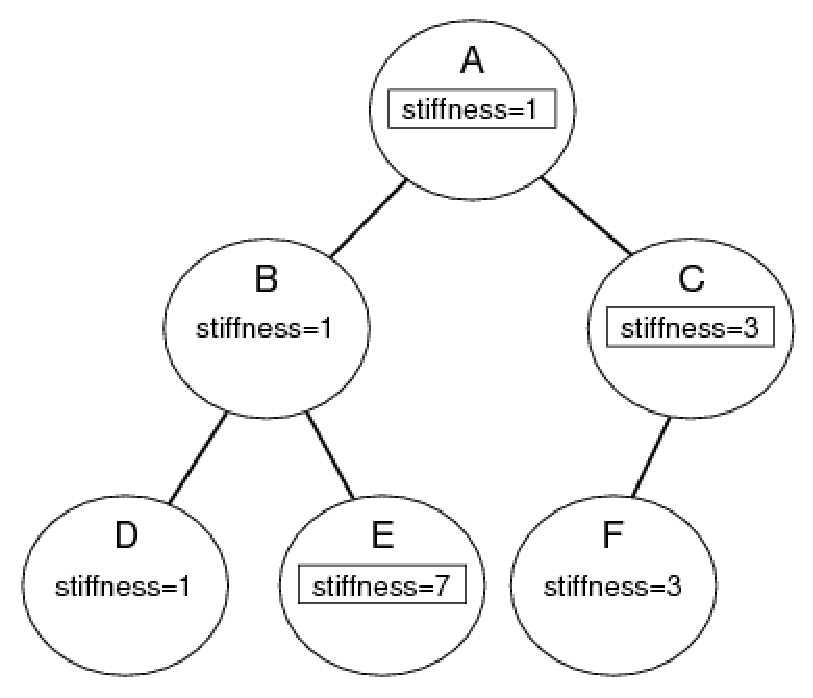
\includegraphics[]{images/inheritance}
\else
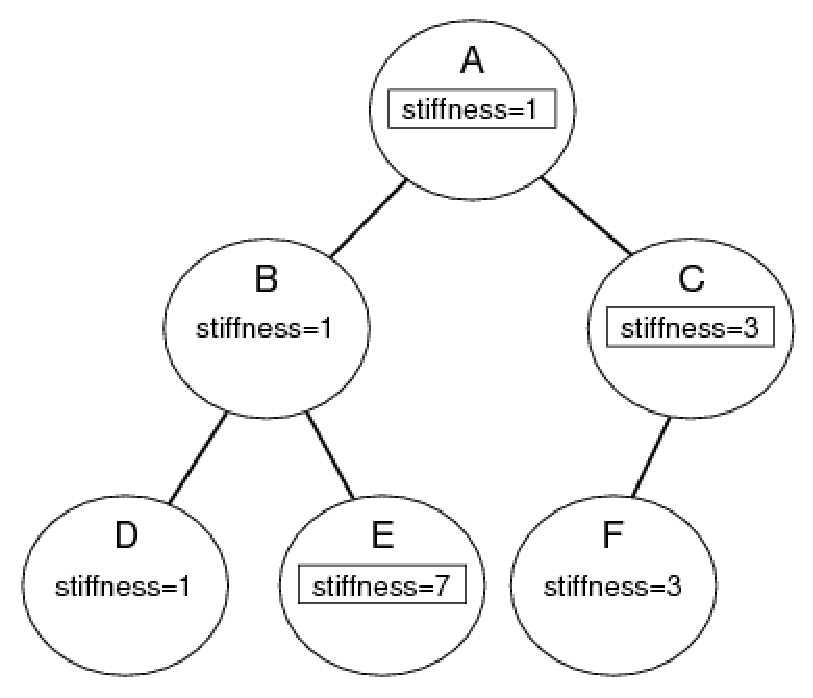
\includegraphics[height=2.5in]{images/inheritance}
\fi
\end{center}
\caption{Inheritance of a property named ``stiffness'' within a
hierarchy of property-exporting objects. Explicitly set instances of
the property are surrounded by square boxes.}%
\label{inheritFig}
\end{figure}

Another common use of property inheritance is in setting render
properties: we might like some properties, such as color, to propagate
down to descendant nodes for which a color has not been explicitly
set.

To state things more generally: any property which can be inherited is
called an {\it inheritable} property, and is associated with a mode
whose value is either explicit or inherited. The basic operating
principle of property inheritance is this:

\begin{sideblock}
{\bf Important:}\\
An inherited property's value should equal that
of the nearest matching ancestor property which is explicitly set.
\end{sideblock}

Other behaviors include:

\begin{itemize}

\item Setting a property's value (using either the set accessor in the host
or the {\it set} method of the {\tt Property} handle) will cause its
mode to be set to {\it explicit}.

\item A property's mode can be set directly. When set to explicit, all
descendant nodes in the hierarchy are updated with the property's
value. When set to inherited, the property's value is reset from the
first explicit value in the ancestry, and then propagated to the
descendants.

\item When a new node is added to the hierarchy, all inherited properties
within the node are updated from the ancestry, and then propagated to
the descendants.

\end{itemize}

If a property is inheritable, then the {\tt isInherited()}
method in its {\tt PropertyInfo} structure will return true,
and it's property handle will be an instance of 
{\tt InheritableProperty}:
\begin{lstlisting}[]
interface InheritableProperty extends Property
{
   // sets the property's mode
   public void setMode (PropertyMode mode);

   // returns the property's mode
   public PropertyMode getMode();
}    
\end{lstlisting}
Valid modes are {\tt PropertyMode.Explicit}, 
{\tt PropertyMode.Inherited}, and {\tt PropertyMode.Inactive}. The latter
is similar to {\tt Inherited}, except that setting an {\tt Inactive}
property's value will {\it not} cause its mode to be set to 
{\tt Explicit} and its new value will not be propagated to hierarchy
descendants.

The hierarchy structure which we have been describing is implemented by
having host classes which correspond to hierarchy nodes implement the
{\tt HierarchyNode} interface.
\begin{lstlisting}[]
interface HierarchyNode 
{
   // returns an iterator over this node's children
   Iterable<? extends HierarchyNode> getChildren();

   // returns true if this node has children
   boolean hasChildren();
 
   // returns the parent of this node, if any
   HierarchyNode getParent();   
}    
\end{lstlisting}

These methods should be implemented as wrappers to the underlying
hierarchy implementation.

\section{Exporting Inheritable Properties}

The property package provides most of the code required to make
inheritance work, and so all that is required to implement an
inheritable property is to provide some simple template code within
its exporting class. We will illustrate this with an example.

Suppose we have a property called ``width'' that is to be made
inheritable.  Then addition to it's value variable and set/get
accessors, the host class should provide a {\tt PropertyMode} variable
along with set/get accessors:
\begin{lstlisting}[]
   int myWidth;
   PropertyMode myWidthMode = PropertyMode.Inherited;
   
   public PropertyMode getWidthMode() {
      return myWidthMode;
   }

   public void setWidthMode (PropertyMode mode) {
      myWidthMode = PropertyUtils.setModeAndUpdate (
         this, "width", myWidthMode, mode);
   }
\end{lstlisting}
The call to {\tt PropertyUtils.setModeAndUpdate()} inside the 
{\tt set} method ensures that inherited values within the hierarchy are
properly whenever the mode is changed. If the mode is set to 
{\tt PropertyMode.Explicit}, then the property's value needs to be
propagated to any descendent nodes for which it is inherited.  If the
mode is set to {\tt PropertyMode.Inherited}, then the property's value
needs to be obtained from the ancestor nodes, and then also propagated
to any descendent nodes for which it is inherited.

As mentioned in the previous section, explicitly setting a property's
value using the {\tt set} accessor should cause it's property mode to
be set to {\tt Explicit} and the new value to be propagated to
hierarchy descendents.  This can be accomplished by using 
{\tt PropertyUtils.propagateValue} within the {\tt set} accessor:
\begin{lstlisting}[]
   public void setWidth (int w) {
      myWidth = w;
      myWidthMode = PropertyUtils.propagateValue (
         this, "width", myWidth, myWidthMode);
   }     
\end{lstlisting}

The actual creation of an inherited property can be done using the
{\tt PropertyList} methods
\begin{lstlisting}[]
   void addInheritable (
      String nameAndMethods, String description, 
      Object defaultValue)
    
   void addInheritable (
      String nameAndMethods, String description, 
      Object defaultValue, String options)
\end{lstlisting}
instead of the {\tt add} or {\tt addReadOnly} methods. The {\tt nameAndMethods}
argument may now specify up to five method names, corresponding, in
order, to the get/set accessors for the property value, the getRange
accessor, and the get/set accessors for the property's mode.  If any
of these are omitted or specified as '{\tt *}', then the system
searches for names of the form
{\tt getXxx}, {\tt setXxx}, {\tt getXxxRange}, {\tt getXxxNode}, 
and {\tt setXxxMode}, where
{\tt xxx} is the property name.

Finally, the host objects which actually correspond to hierarchy nodes
must implement the {\tt HierarchyNode} interface as described in the
previous section, {\it and} any routine which adds a node to the
hierarchy must also implement the following code fragment:
\begin{lstlisting}[]
   public void addChild (HierarchyNode node) {
      ... add node to the hierarchy ...
      PropertyUtils.updateInheritedProperties (node);
   }      
\end{lstlisting}
This ensures that when a node is added, all property values within and
beneath it are made consistent with the inheritance hierarchy.

\section{Inheritable and Composite Properties}

Property inheritance is not currently implemented for 
{\tt CompositeProperty} objects, in order to avoid confusion of the
inheritance rules. Suppose a class exports a composite property 
{\tt A}, which in turn exports an inheritable property {\tt B}.  Now
suppose that {\tt A} is an inheritable property with its mode is set
to {\tt Inherited}. Then the entire structure of A, including the
value of B and its mode, is inherited, and it is no longer possible to
independently set the value of B, even if its mode is Explicit.

However, the leaf nodes of a composite property tree certainly can be
inherited. Suppose a class {\tt ThisHost} exports properties 
{\tt width}, {\tt order}, and {\tt renderProps}, and that the latter is a
composite property exporting {\tt width}, {\tt color}, and {\tt size}.
The leafs nodes of the composite property tree exported
by {\tt ThisHost} are the properties
\begin{lstlisting}[]
   width
   order
   renderProps.width
   renderProps.color
   renderProps.size
\end{lstlisting}
Each of these may be inheritable, although {\tt renderProps} may not be. 

It should be noted that all the leaves in a composite property tree
are considered to be unique properties and do not affect each other
with respect to inheritance, even if some of the sub-component names
are the same. For instance, in the above example, the properties 
{\tt width} and {\tt renderProps.width} are different; each may inherit,
respectively, from occurrences of {\tt width} and 
{\tt renderProps.width} contained in ancestor nodes, but they do not affect
each other. This is illustrated by Figure \ref{compositesFig}.

\begin{figure}
\begin{center}
\iflatexml
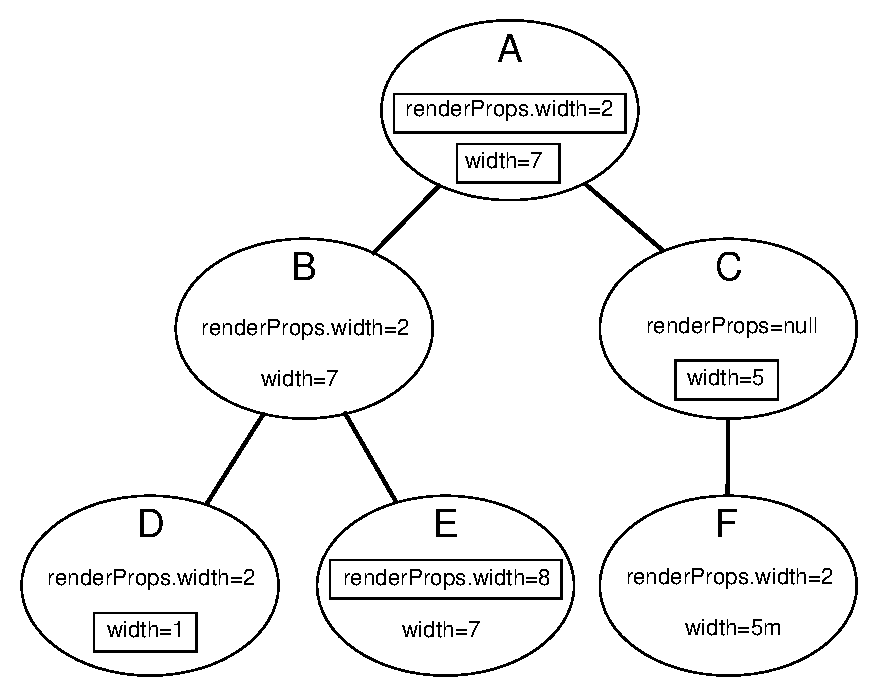
\includegraphics[]{images/composites}
\else
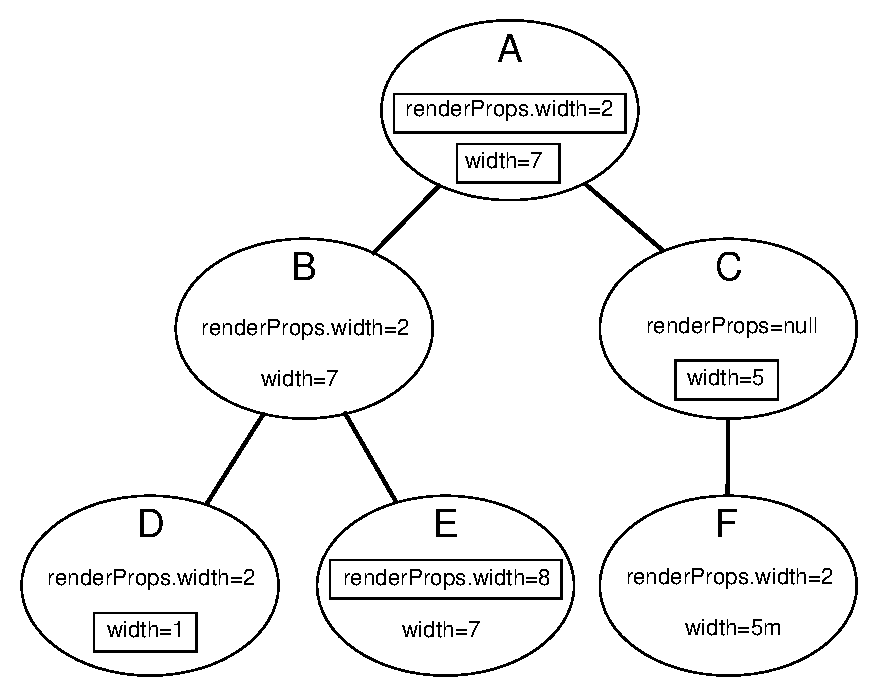
\includegraphics[height=2.5in]{images/composites}
\fi
\end{center}
\caption{Inheritance of the properties {\tt width} and {\tt
renderProps.width} within a hierarchy}%
\label{compositesFig}
\end{figure}

Also, if a CompositeProperty is set to {\tt null} within a particular
node, then the inheritance of its sub-properties passes straight
through that node as though the property was not defined there at
all. For example, in Figure \ref{compositesFig}, {\tt renderProps} is
set to {\tt null} in node C, and so {\tt renderProps.width} in node F
inherits its value directly from node A.

Composite property inheritance is fully supported if an inheritable
property's {\tt set} accessor invokes 
{\tt PropertyUtils.update\-CompositeProperty} as shown in the code example at
the end of Section \ref{compositeSec}.

